\documentstyle[cec2003,multicol,times,epsfig]{article}

\begin{document}
\pagestyle{empty}
\sloppy

\twocolumn[
\title{SimME\\Mobile Multiplayer Gaming}

% list of authors with occupation
\vspace{2mm}
\begin{multicols}{4}
\begin{center}
	Wolfgang Slany\\
	\emph{Project Lead}\\
	wsi@ist.tugraz.at
\end{center}
\begin{center}
	Kariem Hussein\\
	\emph{Architecture and Design}\\
	kariem@users.berlios.de
\end{center}
\begin{center}
	Georg Spielmann\\
	\emph{User Interface}\\
	schurli@users.berlios.de
\end{center}
\begin{center}
	Paul Sprenger\\
	\emph{Technical Documentation}\\
	sprenger@sbox.tugraz.at
\end{center}
\end{multicols}
\vspace{0.25in}
] % end of the argument to \twocolumn

\begin{abstract}

	This paper presents SimME, a multiplayer game for mobile devices (mobile
	phones, PDAs, ...), based on Ramsey's theory. Mobile devices usually have
	limited resources, small displays, and software development poses a
	challenge, even to experienced programmers. SimME a.k.a. Hexi was first
	introduced as a java applet implementation, and is available at
	\textit{\mbox{http://www.dbai.tuwien.ac.at/proj/ramsey/}}. The SimME project
	aims at providing an extensible platform for multiplayer games over the
	Internet on mobile phones and similar devices.

\end{abstract}


\section{Introduction}

	A lot of game developers, particulary developers working in the area of
	wireless communication, are confronted with the same problem: a two player
	game is usually limited to a point-to-point connection (infrared or
	bluetooth communication), depending on the device capabilities. A
	server-based implementation on mobile devices for multiplayer gaming is
	unlikely, due to limited resources.

	The SimME platform provides an extensible set of classes to ease the
	development of simple multiplayer games for mobile devices. The
	communication is based on internet technologies, a domain where most mobile
	device vendors focus their development.

	As a game needs information exchange, the two participating parties have to
	agree on a common protocol. The main purpose of the SimME server is to act
	as a match-making provider. Clients connect to the server to choose their
	opponent. The game is "managed" by the server, i.e. the server creates the
	game and sends meta-information to the clients. See section
	\ref{sec:architecture} for details.

	Figure \ref{fig:communication} shows how users can play SimME over the
	internet.

	\begin{figure*}[htbp]
		\begin{center}
			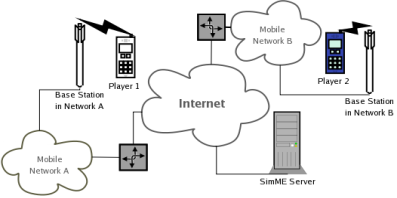
\includegraphics{pics/communication-small.png}
			\caption{Communication between clients on two different networks}
			\label{fig:communication}
		\end{center}
	\end{figure*}


\section{Applied Theory - Ramsey's Theorem}

	The game's rules build on Ramsey's theorem \cite{wiki}. A close analysis of
	the relation between the game and the underlying Ramsey theory can be found
	in \cite{slany_paper}.

	SimME is based on the \emph{Party Puzzle} which describes the following
	problem: Given a set of 6 people at a party, how many people do need to
	randomly select, so that either 3 of them know one another, or 3 of them
	don't know each other. The answer to this question corresponds to the Ramsey
	number R(3,3) = 6.

	Let's call them \emph{A}, \emph{B}, \emph{C}, \emph{D}, \emph{E}, \emph{F}
	and \emph{G}, so that we only have to consider 2 cases:

	\begin{enumerate}

		\item In the first case, suppose A knows three (or more) of the
		others, say, B, C and D. If either B and C, B and D, or C and D are
		mutual acquaintances, then A and the acquainted pair make three
		people who know one another. Otherwise B, C and D are mutual
		strangers.

		\item In the second case, suppose A knows only two (or fewer) of the
		others, say, B and C. If either D and F, D and E, or E and F are
		strangers, then A and the unacquainted pair make three people who do
		not know one another. Otherwise D, E and F are mutual acquaintances.

	\end{enumerate}

	This puzzle can be illustrated by SimME, where the 6 people are represented
	by 6 vertices at the corners of a hexagon. The relationship between two
	people -- strangers or acquaintances -- is represented by coloured edges
	between the corresponding vertices.


\section{Description of the Game}

	The game board consists of six nodes, arranged at the corners of a hexagon.
	Each node is connected to the five other points. At each turn, one player
	connects two points. The first player who interconnects three points with a
	triangle loses the game.

	Figure \ref{fig:gameboard} shows an empty game board on the client device.
	As the game progresses, each move is indicated by painting an edge in the
	player's colour. As there is an odd number of connectable edges, the game
	can never end in a draw.

	\begin{figure}[h]
	\begin{center}
		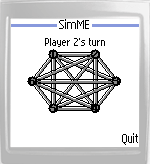
\includegraphics{pics/simme-screen.png}
		\caption{Initial SimME game board on mobile phone}
		\label{fig:gameboard}
	\end{center}
	\end{figure}

\section{Current State of Development}

	Currently SimME supports a \emph{one-player}, \emph{local multi-player} and an
	\emph{internet-based multiplayer} mode.

	\begin{description}

		\item [\textit{One player game (against a computer opponent)}]

			A computer opponent is implemented. As described in section
			\ref{sec:ci} at this time there is no \textit{intelligent} computer
			opponent integrated in the game SimME, but an opponent taking
			randomised turns.

			A learning computer opponent, as implemented in the java applet of
			the game HEXI \cite{slany_paper}, is planned for a future version. .

		\item [\textit{Local multiplayer game (two players - one device)}]

			This playing mode allows two players to play a local game against
			each other, sharing one mobile device.

		\item [\textit{Multiplayer game (with an external game server)}]

			Two human players connect to a game server, using their mobile
			device. This server is responsible for match-making, as there are
			usually more than only two people connected.

			This multiplayer mode is based on the single player mode. The
			opponent replaces the computer player. Instead of waiting for the
			computer player, the game transparently exchanges information with
			the server, and shows the results after receiving the opponent's
			move.

			In the current implementation all communication passes the server.

	\end{description}



\section{Design and Architecture} \label{sec:architecture}

	Optimal extensibility (simple development of future games) is ensured by
	strictly separating game logic and communication.

	The game server can be seen as a sole mediator between the game clients. It
	has no direct access to the client's game logic, though it uses the client
	classes to verify correct gameplay, and to log the game as it progresses.

	The game may be played between players on different continents. Figure
	\ref{fig:communication} shows an example of two players using their mobile
	phones to connect to the Internet, in order to play a game of SimME.

	\subsection{Game Interface Reuse} \label{sec:interface}

		The task is to create a simple interface, used by the server and the
		client to communicate with each other.

		How to build this interface? In a first step, the game's logic is
		abstracted. This abstract representation is used for single player and
		multiplayer games on the client. The single player game extends the
		abstract game with simple AI logic, while a multiplayer game
		implementation (\emph{network aware}) that uses the Internet adds
		transparent network communication. The SimME server uses the abstract
		representation of the game and creates a \emph{managed game} two
		competing clients. This is illustrated in figure \ref{fig:interface}.

		\begin{figure}[h]
		\begin{center}
			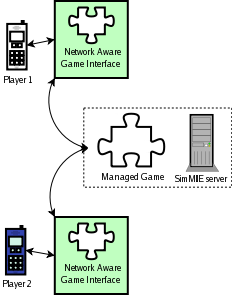
\includegraphics{pics/interface-usage.png}
			\caption{General game implementation: server manages a multiplayer game}
			\label{fig:interface}
		\end{center}
		\end{figure}

		Whenever a move at player 1's mobile phone is performed, the managed
		game is updated accordingly. Player 2's mobile phone receives updated
		game information, and consequently updates its "local" game. Effectively
		the game is transparently played at three locations. The game logic
		implementation, used by all parties, does not allow illegal or duplicate
		moves to be performed.

		It is guaranteed that no redundant information is transferred. The
		clients and the server "know" about the correct state of the game at
		every point in time.

	\subsection{Communication between client and server}

		There are two different implementations employed for the client server
		communication. The client sends direct HTTP requests to the web
		application running on the server. The server's answer is more
		structured, and contains XML content. Figure \ref{fig:com_client_server}
		illustrates this.

		\begin{figure}[h]
		\begin{center}
			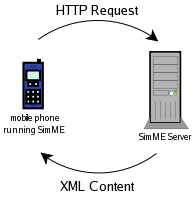
\includegraphics{pics/com_client_server.png}
			\caption{Communication between client and server}
			\label{fig:com_client_server}
		\end{center}
		\end{figure}

		The communication interface is backed by dynamic menus, created and
		administrated by the game server. The menus are used to create a dynamic
		user interface at the client side, comparable to very simple HTML or WML
		pages.

		These dynamic menus can be reused by other games because they are
		organised in interface classes and consequently are modular. The layout
		and content is defined in XML and can be exchanged at run-time.

	\subsection{Internal administration on the server}

		The server's web application serializes the data in a relational
		database. Currently running games are only represented in the server's
		application memory. Information about registered players and completed
		games are saved to the database. The same database will be used for
		future games being implemented on the SimME-platform.

		Information about currently registered and online players, games in
		progress etc., can be accessed with a web browser.


\section{Computational Intelligence} \label{sec:ci}

	The current implementation of SimME does not provide a player with
	computational intelligence. SimME's predecessor, the java applet Hexi
	\cite{slany_paper} (available at
	\textit{http://www.dbai.tuwien.ac.at/proj/ramsey/}), provides a learning
	computer opponent.

	\subsection{CI Player for SimME}

		Based on that implementation a CI gaming unit will be integrated in the
		game SimME, on the client as well as on the server side. By implementing
		the gaming unit at the SimME server, it is possible to record statistics
		as basis for game strategies. Game matches could be logically analysed
		to further improve these strategies.

		This is not limited to games against the computer, it even supports the
		analysis of matches between two human players.

		The CI gaming unit's difficutly can be adjusted to the player's gaming
		level, to provide just enough competition for new and experienced
		players.


\section{Outlook}

	In this section some ideas are listed that we will implement in the future.

	\subsection{Player communication during a running game}

		Like Tony Manninnen says in "Interaction Forms and Communicative Actions
		in Multiplayer Games" \cite{mann03}:

		\begin{quotation}

			Rich interaction is achieved through direct manipulation of objects,
			multimodal input devices and the high number of degrees of freedom.
			However, this relatively technical definition covers only one
			portion of the concept. In addition to these, social, cultural and
			communicative aspects have a significant impact on interaction
			richness. [\ldots]

			\textit{Rich interaction does not necessarily require rich
			interfaces.}

		\end{quotation}

		The last sentence matches our approach to useful communication forms
		between players. The idea is to provide a set of \emph{fixed} phrases
		which can be sent to the opponent player during gameplay. This approach
		is a time saving way to communicate with the opponent.

		Communication between players is important, in order to maintain a
		stable user base. As a mobile phone does not provide very much space for
		communication while showing the game board, several pre-defined phrases
		will be very usefull for the players. The phrases can even be localized,
		so that a French player sends "Bien jou\'e" and his English speaking
		opponents receives "Good Game".

		It is also planned to implement chat functionality for more flexible
		communication.

	\subsection{Integration of a CI gaming unit}

		As described in section \ref{sec:ci} a CI gaming unit will be integrated
		in the SimME server and optionally on client side. On a mobile device
		this unit may exceed space restrictions. This unit supports a
		challenging single player game mode one the one hand, and improves the
		value of game statistics on the other hand.

		The CI gaming unit implemented by Wolfgang Slany is a learning opponent,
		so the recorded games will be used by the CI gaming unit to improve the
		its performance.

	\subsection{Game statistics}

		A ranking system among users with sophisticated performance statistics
		will be implemented to raise user satisfaction. Besides win and loss
		counts these statistics will show the following data:

		\begin{itemize}

			\item Rating based on move effectiveness

			\item Number of moves to win a game

			\item Game length

			\item Move length, which denotes how fast the player executes a move.

		\end{itemize}




\begin{thebibliography}{10}

	\bibitem[mann03]{mann03} Manninen T. (2003) "Interaction Forms and
	Communicative Actions in Multiplayer Games", The international journal of
	computer game research

	\bibitem[slany99]{slany_paper} Slany W. (1999) "Graph Ramsey games",
	Department of Information Systems, Database and Artificial Intelligence
	Group, Technical University of Vienna. An online version of this paper is
	available at
	\textit{http://www.dbai.tuwien.ac.at/ftp/papers/slany/dbai-tr-99-34.ps.gz}

	\bibitem[wiki04]{wiki} Wikipedia.org (2004) "Ramsey's theorem", Wikipedia --
	The Free Encyclopedia: http://en.wikipedia.org/wiki/Ramsey's\_theorem

\end{thebibliography}

\end{document}
